\section{Evaluation}
\label{sec:evaluation}

To be able to compare the results of different experiments, we have fixed the number of iterations of Stochastic Gradient Descent to a constant value of $20000$.

\subsection{Train Error}
\begin{figure}[t]
	\centering
	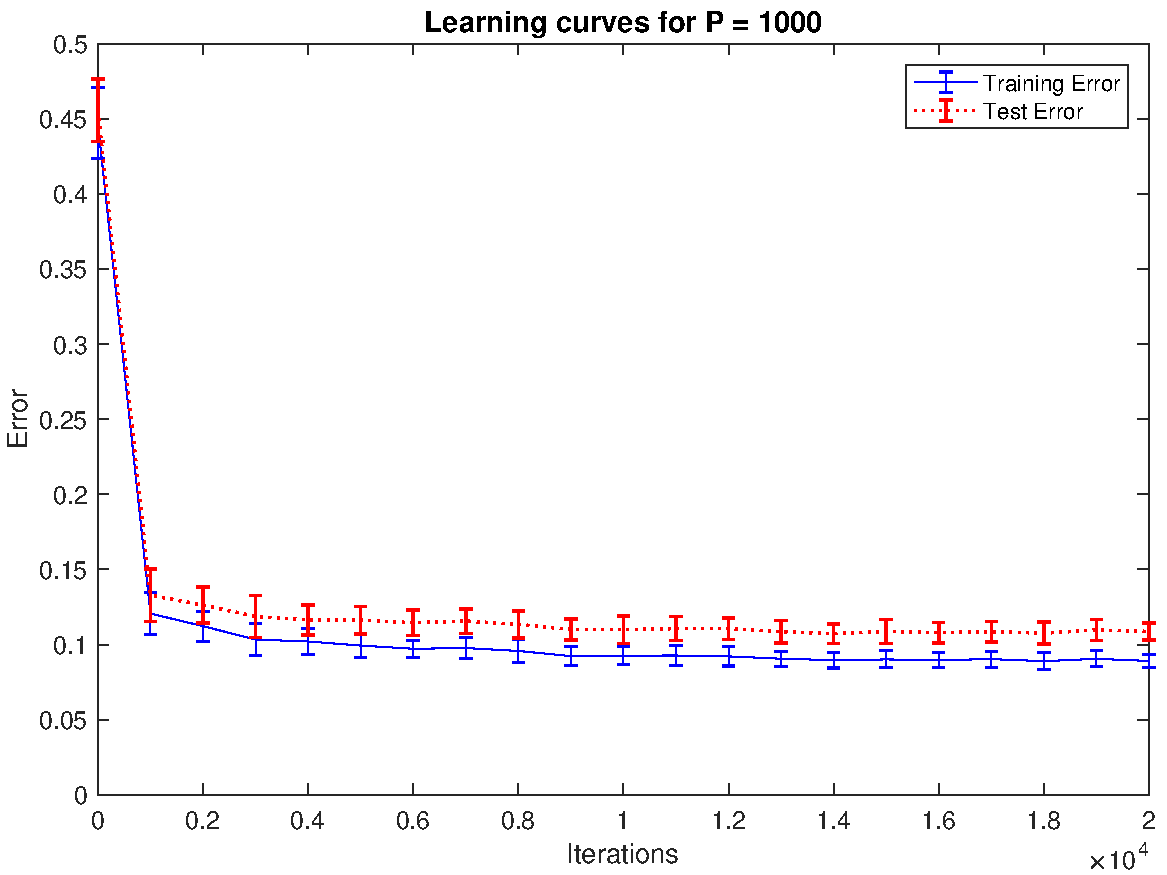
\includegraphics[width=\columnwidth]{figures/error}
	\caption{Train and test error of the network for $P = 1000$. Training executed with a fixed
	learning rate $\eta = 0.05$.}
	\label{fig:training_error}
\end{figure}

\cref{fig:training_error} shows the train and test error for the network trained using Stochastic Gradient Descent on the first $1000$ examples.
Both the train error and test error drop very quickly during approximately the first $1000$ iterations, then remain almost constant for the rest of the training.
The test error is slightly bigger than the train error:
at the end of the training, the train error is around $0.10$ and the test error around $0.12$.
Since the test error never increases, the model does not seem to overfit the training data.

\subsection{Learned Weights}
\begin{figure}[t]
	\centering
	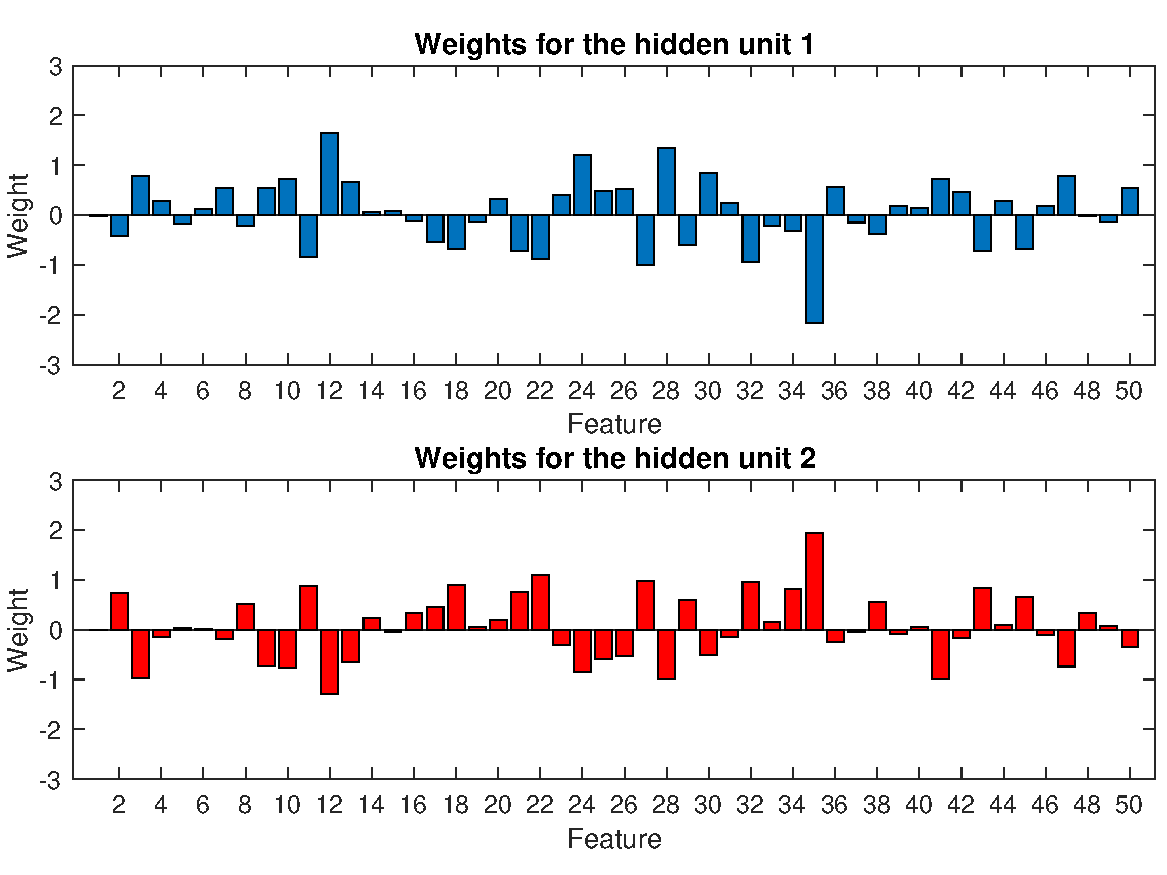
\includegraphics[width=\columnwidth]{figures/weights_p_1000}
    \caption{Weights of the hidden units of the network after the training.}
	\label{fig:weights}
\end{figure}

\cref{fig:weights} shows the weights learned from the hidden units of the networks after the training for $P = 1000$.
As expected, the units learn different weights thanks to the random initialization of the weights.

\subsection{Train Dataset}
\begin{figure}[t]
	\centering
	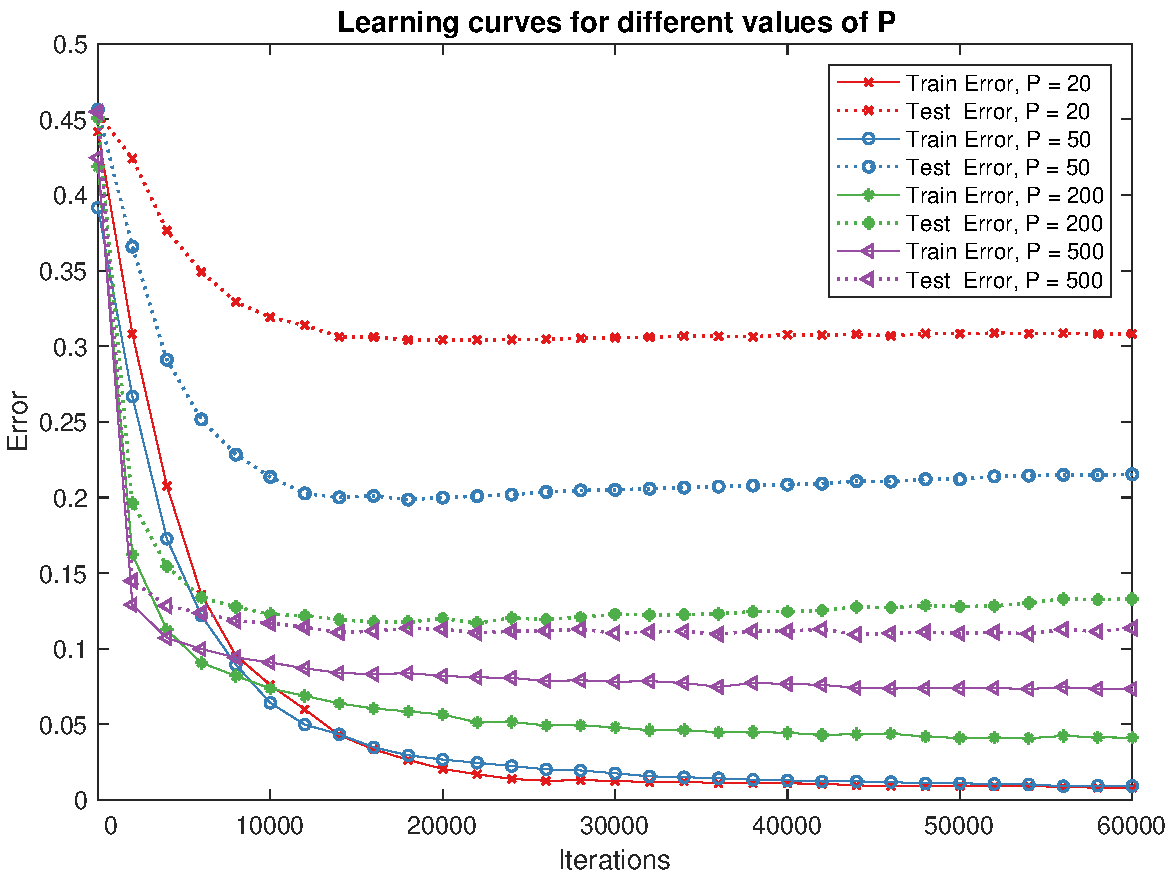
\includegraphics[width=\columnwidth]{figures/error_ps}
	\caption{Train and test error of the network for different numbers of training examples $P$. Trainings executed with a fixed learning rate $\eta = 0.05$.}
	\label{fig:ps}
\end{figure}

\cref{fig:ps} shows the train and test error for different values of $P$, i.e. for a network trained on training dataset of different dimensions.
For very small training datasets ($P = 20$, $P = 50$), the train error drops very quickly and stabilizes close to $0$;
the test error is high and even increases during the training for $P = 50$.
It seems like the network does not see enough examples to generalize properly to new data and tends to overfit the train set.

For $P = 200$, the train error is higher, but the test error gets significantly smaller.
Still, the test error increases during the training, which indicates overfit.

For $P = 500$, the train and test error get closer and remain constant during most of the training.
The results for higher values of $P$ are really similar and are thus not shown.

\subsection{Train Policy}
The learning rate influences the number of iterations the training algorithm needs to converge to the optimal weights.
A high learning rate causes the process to be unstable while a low one takes too long time to converge.
For this reason, we implement different schedulers for the learning rate able to change its value over time as a function of the iteration: \textit{fixed}, \textit{step}, \textit{exponential} and \textit{cycle}.
\cref{fig:learning_rates_policies} shows how they change the learning rate over time.
From the application of these \acp{LRP} we expect a change in the behavior of the error function.
In most \acp{LRP} the learning rate decreases with time, so the error should get more stable.

\begin{figure}
	\centering
	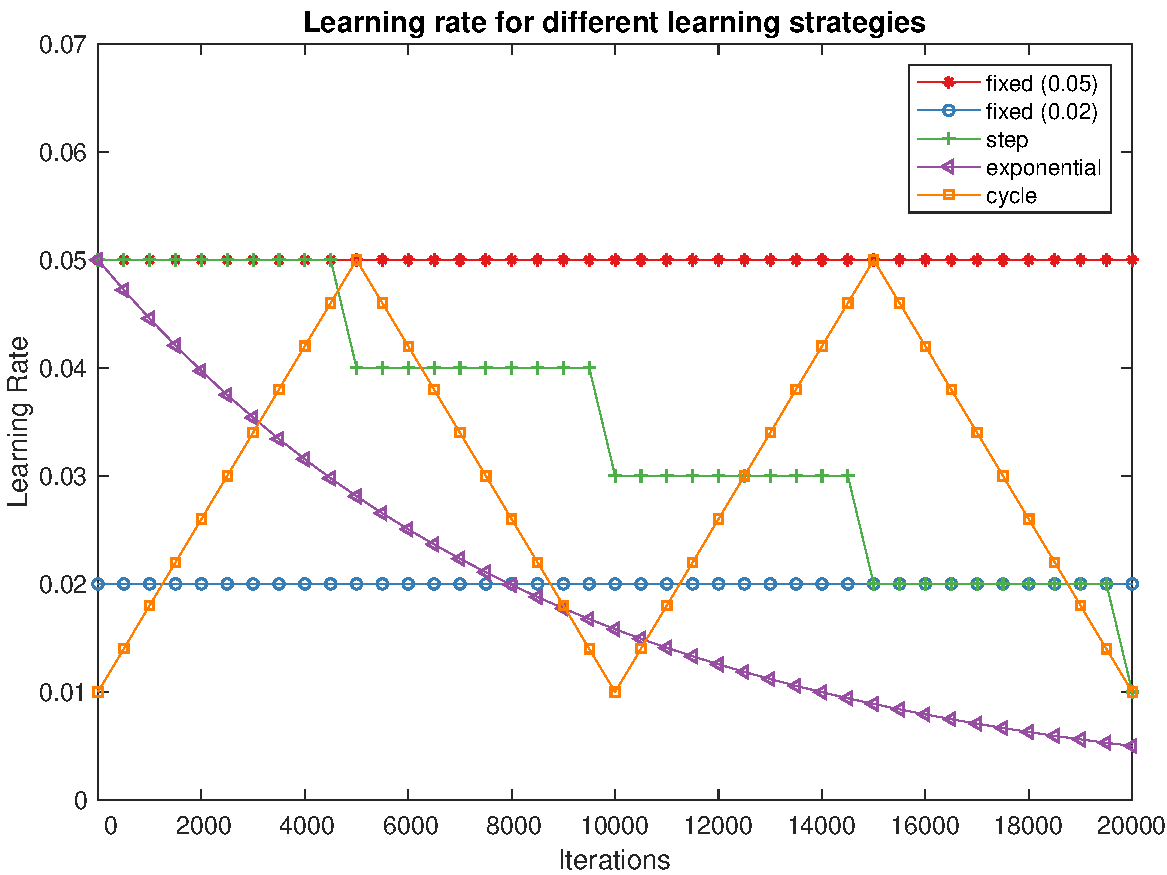
\includegraphics[width=\columnwidth]{figures/learning_rates}
	\caption{Learning rate evolution over iterations for different learning rate policies.}
	\label{fig:learning_rates_policies}
\end{figure}

\cref{fig:lrp_training_error} shows that different \acp{LRP} have different effects on the error trend.
Overall, all implemented \acp{LRP} perform better than the \textit{fixed}($0.05$).
The next sections discuss them in more detail.

\begin{figure}
	\centering
	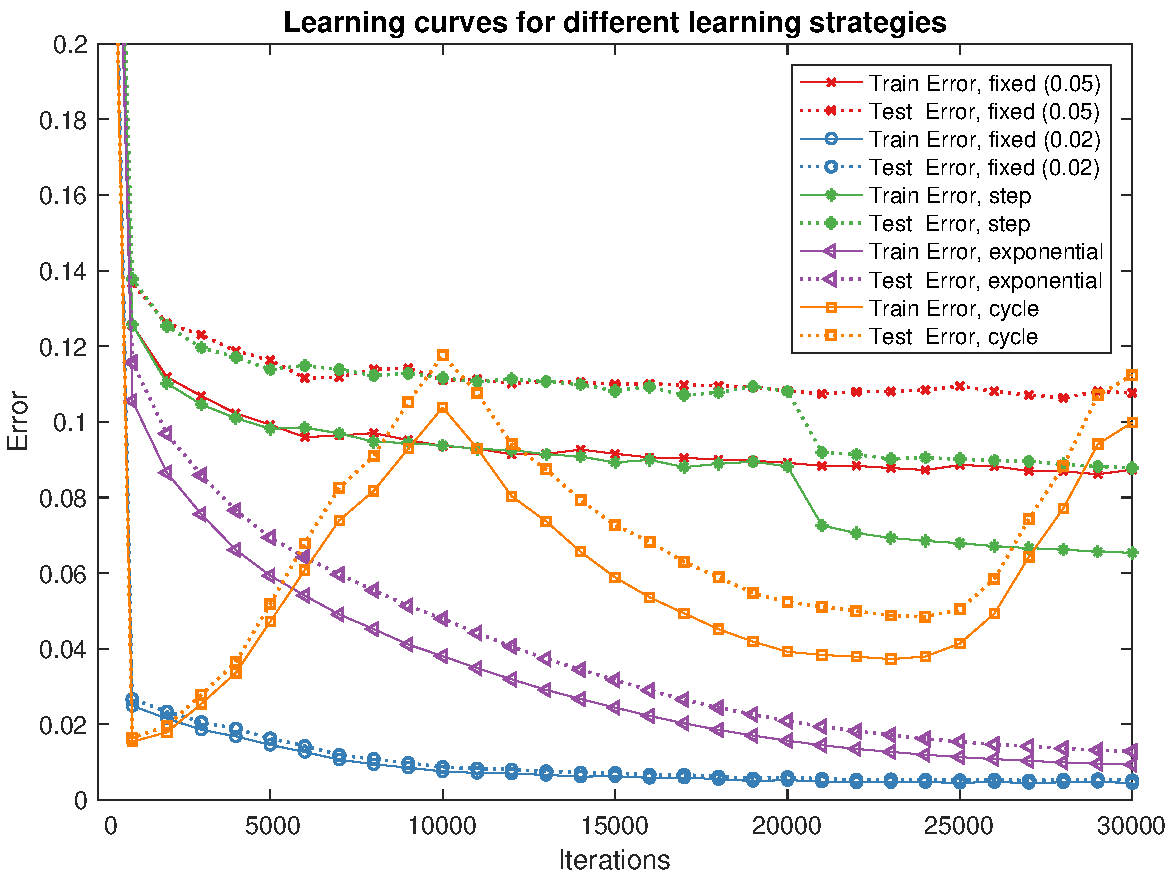
\includegraphics[width=\columnwidth]{figures/error_strategies}
	\caption{Training and test error for different learning rate policies.}
	\label{fig:lrp_training_error}
\end{figure}

\subsubsection{Fixed \ac{LRP}}
As the name suggests this \ac{LRP} leaves the learning rate fixed during iterations.
The error to drops down after around $500$ iterations, then decreases very slowly. 
On our dataset, this strategy has the best performances with a learning rate $\eta = 0.02$.

\subsubsection{Step \ac{LRP}}
This strategy consists in decreasing the learning rate of a defined quantity (\textit{drop}) after a certain number of iterations (\textit{step\_size}).
As shown in \cref{fig:learning_rates_policies}, we chose \textit{step\_size} = $5000$ and \textit{drop} = $0.01$.
\cref{fig:lrp_training_error} shows a drop in both train and test error close to the step in the learning rate.

\subsubsection{Exponential \ac{LRP}}
This strategy consist in decreasing the learning rate in an exponential way, i.e. in dividing it by a constant value at each iteration.
This \ac{LRP} lets the network learn quickly in the beginning, when the weights are still far from the teacher, and slowly while they are getting closer to it.
\cref{fig:lrp_training_error} shows a smoother decrease of both the train and test errors, which just after $3000$ iterations tends to have a value smaller than $0.1$.

\subsubsection{Cycle}
This strategy consists in increasing and decreasing the learning rate linearly over the number of iterations, creating a sawteeth plot as shown in \cref{fig:learning_rates_policies}.
The aim of this \ac{LRP} is to avoid local minima letting the value of the learning rate to grow again when it reaches its minimum value.
\cref{fig:lrp_training_error} shows that with the data provided the \ac{LRP} performs well as far as the value of the learning rate is smaller than the \textit{fixed}($0.02$) one, then the error increases following the increase of the learning rate and never goes back to its early low value.
